\documentclass[a4paper, 10pt]{article}
\usepackage[utf8]{inputenc}
\usepackage[spanish]{babel}
\usepackage{graphicx}
\usepackage{geometry}
\usepackage{listings}
\usepackage{amsmath}
\usepackage{amsfonts}
\usepackage{amssymb}
\usepackage{caratula}

\newcommand{\Z}{\mathbb{Z}}
\def\code#1{\texttt{#1}}
\newcommand\tab[1][0.5cm]{\hspace*{#1}}

\geometry{a4paper, margin=0.7in}

\begin{document}
    %Caratula
    \pagenumbering{gobble}
    \newpage

    \begin{center}
        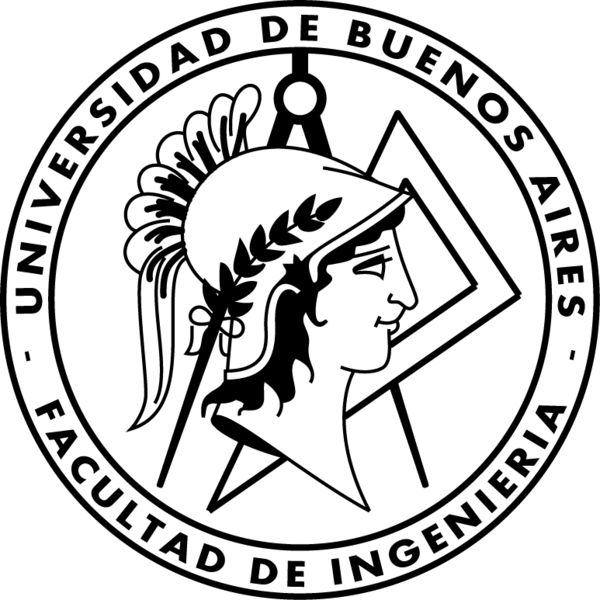
\includegraphics[width=5cm, height=5cm]{images/logo}
    \end{center}

    \materia{Teoría de Algoritmos I}
    \submateria{Primer Cuatrimestre 2017}
    \titulo{Trabajo Práctico 3}

    \integrante{Rodrigo De Rosa}{97799}{rodrigoderosa@outlook.com}
    \integrante{Marcos Schapira}{---}{schapiramarcos@gmail.com}
    \integrante{Facundo Guerrero}{97981}{facundoiguerrero@gmail.com}
    \maketitle
    %Fin caratula
    %Table of contents
    \newpage
    \pagenumbering{roman}
    \tableofcontents
    %Fin table of contents
    %Informe
    \newpage
    \pagenumbering{arabic}

    \section{Programación Dinámica}
        En esta sección se analiza una solución al problema de la predcción de acciones a través
        de la programación dinámica.
        \subsection{Algoritmo}
            El algoritmo utilizado para resolver el problema planteado fue %.....
            \subsubsection{Funcionamiento}
                Este algoritmo funciona de la siguiente forma:
                \begin{itemize}
                    \item Determina un \code{día de compra}, un \code{día de venta}, un \code{día de compra auxiliar},
                    una \code{ganancia máxima} y una \code{ganancia temporal}.
                    \item Itera sobre todos los días (valores diferentes de acciones) verificando si
                    en el día actual es más o menos favorable comprar acciones que en el día en el
                    que se pretendía hacerlo hasta el momento, determinando el \code{día de compra auxiliar}.
                    \item A partir del día que determinó, calcula la \code{ganancia temporal} como la que se obtendría
                    si las acciones fueran vendidas el día actual y verifica si es mayor a la \code{ganancia máxima}
                    hasta el momento.
                    \item En tal caso, determina el \code{día de venta} como el actual, el \code{día de compra}
                    como el que previamente era el \code{día de compra auxiliar} y la \code{ganancia máxima} como
                    la que era la \code{ganancia temporal}.
                    \item Al finalizar la iteración, queda determinado el \code{día de compra} más conveniente, el
                    \code{día de venta} más conveniente y la \code{ganancia máxima} obtenible.
                \end{itemize}
            \subsubsection{Ecuación de recurrencia}
                Para la ecuación de recurrencia se plantea lo siguiente: \\
                \begin{itemize}
                  \item Se tiene una variable \code{Ci = Dìa en el que se compran las acciones hasta el paso i, con i = 1, ..., n}.
                  \item Ademas, se tiene otra variable \code{Vk = Dìa en el que se venden las acciones hasta el paso k, con k = i, ..., n}.
                  \item Observar que k esta relacionada con i, ya que el dia de venta debe ser mayor o igual al dia de compra. En el caso de ser igual, la ganancia seria 0.
                  \item Se puede obtener la \code{Ganancia Temporal} del paso \code{i,k}, como \code{GT i,k = Vk - Ci}.
                  \item Entonces, la \code{Ganancia Màxima} es la maxima \code{GT i,k} obtenida al final del algoritmo.
                  \item Se puede definir la \code{ganancia maxima} para el paso \code{i,k} como:
                  \code{GM i,k} =
                  \begin{cases}
                    Vk - Ci  & \mbox{si } GT i,k > GM i,k \\
                    GT i,k-1 & \mbox{si } GT i,k <= GM i,k
                  \end{cases}
                \end{itemize}

    \newpage

    \section{Algoritmos Randomizados}
            En esta sección se analiza una solución al problema de hallar el corte global
        mínimo en un grafo no dirigido a través de un algoritmo randomizado.
        \subsection{Algoritmo}
                Para resolver este problema se utilizó el algoritmo de Karger descripto en
            la bibliografía proporcionada por la cátedra.
            \subsubsection{Funcionamiento}
                Sea el grafo $G = (E, V)$, el procedimiento del algoritmo es el siguiente:
                \begin{itemize}
                    \item Mientras $|V| > 2$:
                    \begin{itemize}
                        \item Se elige $e(u, v) \in E$ aleatoriamente.
                        \item Se crea un $w \in V$, el cual reemplaza tanto a $u$ como a $v$ en todas
                        las aristas en las que se encuentran. Es decir, $w$ puede tener más de una arista
                        que vaya a un mismo vértice $q \in V$.
                        \item Se elimina $e(u, v)$ de $E$.
                        \item Si existe alguna $e(v, v) \in E$ (arista de un vértice consigo mismo), se elimina.
                    \end{itemize}
                    \item Se devuelven las aristas que unen a esos dos vértices como el corte mínimo.
                \end{itemize}
            \subsubsection{Categoría de randomización}
                    Es un algoritmo \emph{Monte-Carlo} porque para algún orden de selección aleatoria
                de aristas, el corte obtenido \emph{no} es el mínimo. Es decir, es rápido siempre pero no siempre
                da resultados correctos. \\
                \tab La probabilidad de que este algoritmo devuelva un corte que sea mínimo es $p \geqslant \binom{n}{2}^{-1}$
                con $n = |V|$. Un dato adicional es que si el algoritmo se corre $T = \binom{n}{2}\ln{n}$ veces,
                la probabilidad de no encontrar un corte mínimo es $[1-p]^T \leqslant \dfrac{1}{n}$ en un tiempo
                $O(Tm) = O(n^2m\log{n})$ con $m = |E|$.
    \newpage

    \section{Algoritmos Aproximados}
        \tab En esta sección se analiza una solución al problema de la suma de subconjuntos
        a través de un algoritmo aproximado.
        \subsection{Algoritmo}
            \tab Para resolver este problema se utilizó la estrategia polinómica descripta en
            la bibliografía proporcionada por la cátedra.
            \subsubsection{Funcionamiento}
                \tab Este algoritmo %....
    \newpage

    \section{Ejecución de programas}
    \tab Para correr cada algoritmo, se debe ejecutar el archivo principal de cada uno.
    Esto se hace de la siguiente forma: \\
    \tab\tab En la carpeta \code{Programación Dinámica} abrir la consola y ejecutar \code{python main.py} \\
    \tab\tab En la carpeta \code{Algoritmos Randomizados} abrir la consola y ejecutra \code{python main.py} \\
    \tab\tab En la carpeta \code{Algoritmos Aproximados} abrir la consola y ejecutra \code{python main.py} \\

    %Fin informe
\end{document}
